\documentclass[11pt,twoside,a4paper]{article}
% http://www-h.eng.cam.ac.uk/help/tpl/textprocessing/latex_maths+pix/node6.html symboles de math
% http://fr.wikibooks.org/wiki/Programmation_LaTeX Programmation latex (wikibook)
%=========================== En-Tete =================================
%--- Insertion de paquetages (optionnel) ---
\usepackage[french]{babel}   % pour dire que le texte est en fran{\'e}ais
\usepackage{a4}	             % pour la taille   
\usepackage[T1]{fontenc}     % pour les font postscript
\usepackage{epsfig}          % pour gerer les images
%\usepackage{psfig}
\usepackage{amsmath, amsthm} % tres bon mode mathematique
\usepackage{amsfonts,amssymb}% permet la definition des ensembles
\usepackage{float}           % pour le placement des figure
\usepackage{verbatim}

\usepackage{longtable} % pour les tableaux de plusieurs pages

\usepackage[table]{xcolor} % couleur de fond des cellules de tableaux

\usepackage{lastpage}

\usepackage{fancybox}

\usepackage{multirow}

\usepackage{multicol} % pour {\'e}crire dans certaines zones en colonnes : \begin{multicols}{nb colonnes}...\end{multicols} 

% \usepackage[top=1.5cm, bottom=1.5cm, left=1.5cm, right=1.5cm]{geometry}
% gauche, haut, droite, bas, entete, ente2txt, pied, txt2pied
\usepackage{vmargin}
\setmarginsrb{0.20cm}{0.20cm}{0.20cm}{0.20cm}{15pt}{3pt}{15pt}{3pt}

\usepackage{lscape} % changement orientation page
%\usepackage{frbib} % enlever pour obtenir references en anglais
% --- style de page (pour les en-tete) ---
\pagestyle{empty}

% % % en-tete et pieds de page configurables : fancyhdr.sty

% http://www.trustonme.net/didactels/250.html

% http://ww3.ac-poitiers.fr/math/tex/pratique/entete/entete.htm
% http://www.ctan.org/tex-archive/macros/latex/contrib/fancyhdr/fancyhdr.pdf
% \usepackage{fancyhdr}
% \pagestyle{fancy}
% % \newcommand{\chaptermark}[1]{\markboth{#1}{}}
% % \newcommand{\sectionmark}[1]{\markright{\thesection\ #1}}
% \fancyhf{}
% \fancyhead[LE,RO]{\bfseries\thepage}
% \fancyhead[LO]{\bfseries\rightmark}
% \fancyhead[RE]{\bfseries\leftmark}
% \fancyfoot[LE]{\thepage /\pageref{LastPage} \hfill
	% TITLE
% \hfill 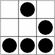
\includegraphics[width=0.5cm]{img/logo_glider.png} }
% \fancyfoot[RO]{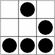
\includegraphics[width=0.5cm]{img/logo_glider.png} \hfill
	% TITLE
% \hfill \thepage /\pageref{LastPage}}
% \renewcommand{\headrulewidth}{0.5pt}
% \renewcommand{\footrulewidth}{0.5pt}
% \addtolength{\headheight}{0.5pt}
% \fancypagestyle{plain}{
	% \fancyhead{}
	% \renewcommand{\headrulewidth}{0pt}
% }

\definecolor{grey25}{gray}{0.75}
\definecolor{grey50}{gray}{0.50}

\def\imgCORPS{\begin{tabular}[h]{p{0.65cm}}\includegraphics[width=0.50cm]{../../../../../../imgGraphics/rolePlayingGame/SimulacreS/normal40x40/corps.png}		\\ \end{tabular}}
\def\imgINSTI{\begin{tabular}[h]{p{0.65cm}}\includegraphics[width=0.50cm]{../../../../../../imgGraphics/rolePlayingGame/SimulacreS/normal40x40/instinct.png}	\\ \end{tabular}}
\def\imgCOEUR{\begin{tabular}[h]{p{0.65cm}}\includegraphics[width=0.50cm]{../../../../../../imgGraphics/rolePlayingGame/SimulacreS/normal40x40/coeur.png}		\\ \end{tabular}}
\def\imgESPRI{\begin{tabular}[h]{p{0.65cm}}\includegraphics[width=0.50cm]{../../../../../../imgGraphics/rolePlayingGame/SimulacreS/normal40x40/esprit.png}		\\ \end{tabular}}

\def\imgPERCE{\begin{tabular}[h]{p{0.65cm}}\includegraphics[width=0.50cm]{../../../../../../imgGraphics/rolePlayingGame/SimulacreS/normal40x40/perception.png}	\\ \end{tabular}}
\def\imgACTIO{\begin{tabular}[h]{p{0.65cm}}\includegraphics[width=0.50cm]{../../../../../../imgGraphics/rolePlayingGame/SimulacreS/normal40x40/action.png}		\\ \end{tabular}}
\def\imgDESIR{\begin{tabular}[h]{p{0.65cm}}\includegraphics[width=0.50cm]{../../../../../../imgGraphics/rolePlayingGame/SimulacreS/normal40x40/desir.png}		\\ \end{tabular}}
\def\imgRESIS{\begin{tabular}[h]{p{0.65cm}}\includegraphics[width=0.50cm]{../../../../../../imgGraphics/rolePlayingGame/SimulacreS/normal40x40/resistance.png}	\\ \end{tabular}}

\def\imgNATUR{\begin{tabular}[h]{p{0.65cm}} \includegraphics[width=0.50cm]{../../../../../../imgGraphics/rolePlayingGame/SimulacreS/normal40x40/naturel.png}	\\  \end{tabular}}
\def\imgHUMAI{\begin{tabular}[h]{p{0.65cm}} \includegraphics[width=0.50cm]{../../../../../../imgGraphics/rolePlayingGame/SimulacreS/normal40x40/humain.png}		\\  \end{tabular}}
\def\imgMATER{\begin{tabular}[h]{p{0.65cm}} \includegraphics[width=0.50cm]{../../../../../../imgGraphics/rolePlayingGame/SimulacreS/normal40x40/material.png}	\\  \end{tabular}}
\def\imgVIRTU{\begin{tabular}[h]{p{0.65cm}} \includegraphics[width=0.50cm]{../../../../../../imgGraphics/rolePlayingGame/SimulacreS/normal40x40/virtuel.png}	\\  \end{tabular}}

\def\imgPUISS{\begin{tabular}[h]{p{0.65cm}} \includegraphics[width=0.50cm]{../../../../../../imgGraphics/rolePlayingGame/SimulacreS/normal40x40/puissance.png}	\\  \end{tabular}}
\def\imgRAPID{\begin{tabular}[h]{p{0.65cm}} \includegraphics[width=0.50cm]{../../../../../../imgGraphics/rolePlayingGame/SimulacreS/normal40x40/rapidite.png}	\\  \end{tabular}}
\def\imgPRECI{\begin{tabular}[h]{p{0.65cm}} \includegraphics[width=0.50cm]{../../../../../../imgGraphics/rolePlayingGame/SimulacreS/normal40x40/precision.png}	\\  \end{tabular}}
\def\imgPOUVO{\begin{tabular}[h]{p{0.65cm}} \includegraphics[width=0.50cm]{../../../../../../imgGraphics/rolePlayingGame/SimulacreS/normal40x40/pouvoir.png}	\\  \end{tabular}}


%============================= Corps =================================
\begin{document}

\begin{tabular}[h]{p{6cm} p{4cm} p{4cm} p{4cm} }
	\begin{tabular}[h]{ p{5.85cm} }
		\includegraphics[width=5.5cm]{../../../../../../imgGraphics/rolePlayingGame/SimulacreS/logos/logoSimulacreSAlternative.png} \\
	\end{tabular}
		&
	\begin{tabular}[h]{ p{4.0cm} }
		{\scriptsize Joueur : }					\\
		\hfill									\\
		Nom : 									\\
		Nationalit{\'e} : 						\\
		M{\'e}tier : 							\\
	\end{tabular}
		&
	\begin{tabular}[h]{ p{4.0cm} }
		{\scriptsize Date de cr{\'e}ation : }	\\
		\hfill									\\
		Sexe : 									\\
		{\^A}ge : 								\\
		Taille, poid : 							\\
	\end{tabular}
		&
	\begin{tabular}[h]{ p{4.0cm} }
		{\scriptsize Joueur : }					\\
		\hfill									\\
		Ph{\'e}notype : 			\newline {\scriptsize \textcolor{grey25}{Peau, yeux, cheveux...} } \\
			 									\\
		%			 							\\
	\end{tabular}
		\\
\end{tabular}

\begin{tabular}[h]{ p{4cm} p{1cm} p{4cm} p{1cm} p{8cm} }
	{\centering \textbf{Composantes}}		& {\scriptsize 3 {\`a} 6 \newline \textcolor{grey25}{(18pts)} }	
	&	{\centering \textbf{Moyens}}		& {\scriptsize 0 {\`a} 4 \newline \textcolor{grey25}{(10pts)} }
	& \textbf{Vie} \textcolor{grey25}{(PV)} \\
	
	\multicolumn{2}{ p{5.00cm} }{ 
		{\footnotesize %
		\begin{tabular}[h]{ p{0.75cm} p{2.5cm} p{0.25cm} p{1.00cm} }
			\arrayrulecolor{grey25}
			\hline %% \cline{4-4}
			\imgCORPS & Corps		& \begin{tabular}[c]{ p{0.20cm} }
			\textcolor{grey25}{\ovalbox{\hfill}} \\ 
			\textcolor{grey25}{\ovalbox{\hfill}} \\ 
			\textcolor{grey25}{\ovalbox{\hfill}} \\
			\end{tabular} & \resizebox{1.0cm}{0.5cm}{ \ovalbox{ \hfill } } \\
			\hline %% \cline{4-4}
			\imgINSTI & Instinct	& \begin{tabular}[c]{ p{0.20cm} }
			\textcolor{grey25}{\ovalbox{\hfill}} \\ 
			\textcolor{grey25}{\ovalbox{\hfill}} \\ 
			\textcolor{grey25}{\ovalbox{\hfill}} \\
			\end{tabular} & \resizebox{1.0cm}{0.5cm}{ \ovalbox{ \hfill } } \\
			\hline %% \cline{4-4}
			\imgCOEUR & C\oe ur		& \begin{tabular}[c]{ p{0.20cm} }
			\textcolor{grey25}{\ovalbox{\hfill}} \\ 
			\textcolor{grey25}{\ovalbox{\hfill}} \\ 
			\textcolor{grey25}{\ovalbox{\hfill}} \\
			\end{tabular} & \resizebox{1.0cm}{0.5cm}{ \ovalbox{ \hfill } } \\
			\hline %% \cline{4-4}
			\imgESPRI & Esprit		& \begin{tabular}[c]{ p{0.20cm} }
			\textcolor{grey25}{\ovalbox{\hfill}} \\ 
			\textcolor{grey25}{\ovalbox{\hfill}} \\ 
			\textcolor{grey25}{\ovalbox{\hfill}} \\
			\end{tabular} & \resizebox{1.0cm}{0.5cm}{ \ovalbox{ \hfill } } \\
			\hline %% \cline{4-4}
		\end{tabular} }
	}	& 
	\multicolumn{2}{ p{5.00cm} }{ 
		{\footnotesize %
		\begin{tabular}[h]{ p{0.75cm} p{2.5cm} p{0.75cm} }
			%% hline %% \cline{4-4}
			\vspace{0.05pt} & & \\
			\imgPERCE &  Perception		 	& \resizebox{1.0cm}{0.5cm}{ \ovalbox{ \hfill } } \\
			%% hline %% \cline{4-4}
			\vspace{0.05pt} & & \\
			\imgACTIO &  Action				& \resizebox{1.0cm}{0.5cm}{ \ovalbox{ \hfill } } \\
			%% hline %% \cline{4-4}
			\vspace{0.05pt} & & \\
			\imgDESIR &  D{\'e}sir			& \resizebox{1.0cm}{0.5cm}{ \ovalbox{ \hfill } } \\
			%% hline %% \cline{4-4}
			\vspace{0.05pt} & & \\
			\imgRESIS &  R{\'e}sistance		& \resizebox{1.0cm}{0.5cm}{ \ovalbox{ \hfill } } \\
			%% hline %% \cline{4-4}
		\end{tabular} }
	}	& \hfill \\

		&	&	&	&	\\

	{\centering \textbf{Domaines}}				& {\scriptsize 0 {\`a} 2 }	
	&	{\centering \textbf{{\'E}nergies}}		& {\scriptsize 0 {\`a} 2 }
	& \hfill \\
	
	\multicolumn{2}{ p{5.00cm} }{ {\scriptsize \textcolor{grey25}{(07pts entre domaines et {\'e}nergies. )} } } 
	&	\multicolumn{2}{ p{5.00cm} }{ {\scriptsize \textcolor{grey25}{(Maximum 1 pour l'{\'e}nergie pouvoir. )} } }
	& \hfill \\
	
	\multicolumn{2}{ p{5.00cm} }{ 
		{\footnotesize %
		\begin{tabular}[h]{ p{0.75cm} p{2.5cm} p{0.75cm} }
			%% hline %% \cline{4-4}
			\imgNATUR &  Naturel		& \resizebox{1.0cm}{0.5cm}{ \ovalbox{ \hfill } } \\
			%% hline %% \cline{4-4}
			\imgHUMAI &  Humain			& \resizebox{1.0cm}{0.5cm}{ \ovalbox{ \hfill } } \\
			%% hline %% \cline{4-4}
			\imgMATER &  Mat{\'e}riel	& \resizebox{1.0cm}{0.5cm}{ \ovalbox{ \hfill } } \\
			%% hline %% \cline{4-4}
			\imgVIRTU &  Virtuel		& \resizebox{1.0cm}{0.5cm}{ \ovalbox{ \hfill } } \\
			%% hline %% \cline{4-4}
		\end{tabular} }
	}	& 
	\multicolumn{2}{ p{5.00cm} }{ 
		{\footnotesize %
		\begin{tabular}[h]{ p{0.75cm} p{2.5cm} p{0.75cm} }
			%% hline %% \cline{4-4}
			\imgPUISS &  Puissance		 				& \resizebox{1.0cm}{0.5cm}{ \ovalbox{ \hfill } } \\
			%% hline %% \cline{4-4}
			\imgRAPID &  Rapidit{\'e}					& \resizebox{1.0cm}{0.5cm}{ \ovalbox{ \hfill } } \\
			%% hline %% \cline{4-4}
			\imgPRECI &  Pr{\'e}cision					& \resizebox{1.0cm}{0.5cm}{ \ovalbox{ \hfill } } \\
			%% hline %% \cline{4-4}
			\imgPOUVO &  \textcolor{grey25}{Pouvoir}	& \resizebox{1.0cm}{0.5cm}{ \ovalbox{ \hfill } } \\
			%% hline %% \cline{4-4}
		\end{tabular} }
	}	& \hfill \\
	
\end{tabular}

~\\

{\scriptsize %
\begin{tabular}[h]{ p{12cm} p{6cm} }
	\textbf{Armes} &  \\
	\begin{tabular}[h]{|p{5.0cm}|p{2.5cm}|p{4.5cm}|}
		\hline
			{\centering \emph{Nom de l'arme} }	&
			{\centering \emph{D{\'e}g{\^a}ts} }	&
			{\centering \emph{Note} }			\\
		\hline
			\dotfill & 
			\textcolor{grey25}{ \ovalbox{ \hfill } } PV, \textcolor{grey25}{ \ovalbox{ \hfill } } PS				& 
			\dotfill	\\
		\hline
			\dotfill	& 
			\textcolor{grey25}{ \ovalbox{ \hfill } } PV, \textcolor{grey25}{ \ovalbox{ \hfill } } PS				& 
			\dotfill	\\
		\hline
			\dotfill	& 
			\textcolor{grey25}{ \ovalbox{ \hfill } } PV, \textcolor{grey25}{ \ovalbox{ \hfill } } PS				& 
			\dotfill	\\
		\hline
	\end{tabular}
	& 
	\begin{tabular}[h]{ p{1.0cm}|p{5.0cm}|}
		\cline{2-2}
		 & \textbf{Divers}		\\
		\cline{2-2}
		 & \dotfill		\\
		\cline{2-2}
		 & \dotfill		\\
		\cline{2-2}
		 & \dotfill		\\
		\cline{2-2}
	\end{tabular}
	\\
\end{tabular} }

\begin{center} {\scriptsize %
\begin{tabular}[h]{ p{3.5cm} p{0.5cm} p{3.5cm} p{0.5cm} p{3.5cm} p{0.5cm} p{3.5cm} p{0.5cm} }
	\multicolumn{8}{ p{18cm} }{ \textbf{\emph{Talents}} }			\\
	%% \hline
		\multicolumn{2}{ p{4.25cm} }{ \resizebox{4.5cm}{0.5cm}{ \ovalbox{ \hfill \textbf{ X} \hfill } } }	&
		\multicolumn{2}{ p{4.25cm} }{ \resizebox{4.5cm}{0.5cm}{ \ovalbox{ \hfill \textbf{-4} \hfill } } }	&
		\multicolumn{2}{ p{4.25cm} }{ \resizebox{4.5cm}{0.5cm}{ \ovalbox{ \hfill \textbf{-2} \hfill } } }	&
		\multicolumn{2}{ p{4.25cm} }{ \resizebox{4.5cm}{0.5cm}{ \ovalbox{ \hfill \textbf{ 0} \hfill } } }	\\
	%% \hline
		\rowcolor[gray]{.75}
		Architecture				\hfill	& \textcolor{grey50}{ \ovalbox{ \hfill } } 
			& \emph{Armes normales}			\hfill	& \textcolor{grey50}{ \ovalbox{ \hfill } } 
			& \emph{Armes l{\'e}g{\`e}res}	\hfill	& \textcolor{grey50}{ \ovalbox{ \hfill } }
			& Athl{\'e}tisme		\hfill	& \textcolor{grey50}{ \ovalbox{ \hfill } } \\
		\rowcolor[gray]{.75}
		Chrirurgie				\hfill		& \textcolor{grey50}{ \ovalbox{ \hfill } } 
			& 					\dotfill	& \textcolor{grey50}{ \ovalbox{ \hfill } } 
			& 					\dotfill	& \textcolor{grey50}{ \ovalbox{ \hfill } }
			& Bagarre				\hfill	& \textcolor{grey50}{ \ovalbox{ \hfill } } \\
		\rowcolor[gray]{.75}
		Droit					\hfill		& \textcolor{grey50}{ \ovalbox{ \hfill } } 
			& 					\dotfill	& \textcolor{grey50}{ \ovalbox{ \hfill } } 
			& 					\dotfill	& \textcolor{grey50}{ \ovalbox{ \hfill } }
			& Chant					\hfill	& \textcolor{grey50}{ \ovalbox{ \hfill } } \\
		%% \rowcolor[gray]{.75}
		Explosifs				\hfill		& \hfill 
			& 					\dotfill	& \textcolor{grey50}{ \ovalbox{ \hfill } } 
			& 					\dotfill	& \textcolor{grey50}{ \ovalbox{ \hfill } }
			& Cuisine				\hfill	& \textcolor{grey50}{ \ovalbox{ \hfill } } \\
		%% \rowcolor[gray]{.75}
		Falsification			\hfill		& \textcolor{grey50}{ \ovalbox{ \hfill } } 
			& Camouflage			\hfill	& \textcolor{grey50}{ \ovalbox{ \hfill } } 
			& \emph{Art \& Artisanat}\hfill	& \textcolor{grey50}{ \ovalbox{ \hfill } }
			& Discr{\'e}tion			\hfill	& \textcolor{grey50}{ \ovalbox{ \hfill } } \\
		%% \rowcolor[gray]{.75}
		Intrusion				\hfill		& \textcolor{grey50}{ \ovalbox{ \hfill } } 
			& Close combat			\hfill	& \textcolor{grey50}{ \ovalbox{ \hfill } } 
			& 					\dotfill	& \textcolor{grey50}{ \ovalbox{ \hfill } }
			& Estimation			\hfill	& \textcolor{grey50}{ \ovalbox{ \hfill } } \\
	
		\rowcolor[gray]{.75}
		\emph{Langues Complexes}	\hfill	& \hfill
			& \emph{Codes \& Usages}\hfill	& \textcolor{grey50}{ \ovalbox{ \hfill } } 
			& 					\dotfill	& \textcolor{grey50}{ \ovalbox{ \hfill } }
			& Langue maternelle		\hfill	& \textcolor{grey50}{ \ovalbox{ \hfill } } \\
		\rowcolor[gray]{.75}
						\dotfill			& \textcolor{grey50}{ \ovalbox{ \hfill } } 
			& 					\dotfill	& \textcolor{grey50}{ \ovalbox{ \hfill } } 
			& Bricolage				\hfill	& \textcolor{grey50}{ \ovalbox{ \hfill } }
			& Ou{\"i}e				\hfill	& \textcolor{grey50}{ \ovalbox{ \hfill } } \\
		\rowcolor[gray]{.75}
						\dotfill			& \textcolor{grey50}{ \ovalbox{ \hfill } } 
			&					\dotfill	& \textcolor{grey50}{ \ovalbox{ \hfill } } 
			& Commerce				\hfill	& \textcolor{grey50}{ \ovalbox{ \hfill } }
			& S{\'e}duction				\hfill	& \textcolor{grey50}{ \ovalbox{ \hfill } } \\
			
		%% \rowcolor[gray]{.75}
		\emph{Pilotage}			\hfill		& \hfill
			& Culture g{\'e}n{\'e}rale		\hfill	& \textcolor{grey50}{ \ovalbox{ \hfill } } 
			& \emph{Conduite}		\hfill	& \textcolor{grey50}{ \ovalbox{ \hfill } }
			& Vue					\hfill	& \textcolor{grey50}{ \ovalbox{ \hfill } } \\
		%% \rowcolor[gray]{.75}
						\dotfill			& \textcolor{grey50}{ \ovalbox{ \hfill } } 
			& {\'E}quitation		\hfill	& \textcolor{grey50}{ \ovalbox{ \hfill } } 
			&  					\dotfill	& \textcolor{grey50}{ \ovalbox{ \hfill } }
			&  					\dotfill	& \textcolor{grey50}{ \ovalbox{ \hfill } } \\
		%% \rowcolor[gray]{.75}
						\dotfill			& \textcolor{grey50}{ \ovalbox{ \hfill } } 
			& \emph{Langues {\'e}trang{\`e}res}\hfill	& \textcolor{grey50}{ \ovalbox{ \hfill } } 
			&  					\dotfill	& \textcolor{grey50}{ \ovalbox{ \hfill } }
			& \multicolumn{2}{ p{4cm} }{ }	\\
		
		\rowcolor[gray]{.75}
		Piratage et Programmes		\hfill	& \textcolor{grey50}{ \ovalbox{ \hfill } } 
			&  					\dotfill	& \textcolor{grey50}{ \ovalbox{ \hfill } } 
			& Dissimulation		\hfill	& \textcolor{grey50}{ \ovalbox{ \hfill } }
			& \multicolumn{2}{ p{4cm} }{ \multirow{10}{4cm}{%
					\ovalbox{ \begin{tabular}[h]{ p{4.0cm} }%
					% \hline%
						\textbf{Points d'Aventure}		\\%
						\hfill	\\%
						\hfill	\\%
						\hfill	\\%
						\hfill	\\%
						\hfill	\\%
					% \hline%
						\textbf{Autres {\'E}nergies}	\\%
						\hfill	\\%
						\hfill	\\%
						\hfill	\\%
						\hfill	\\%
						\hfill	\\%
						\hfill	\\%
						\hfill	\\%
					% \hline%
					\end{tabular} }%
				} } \\
		\rowcolor[gray]{.75}
		\emph{Sciences}			\hfill		& \hfill
			&  					\dotfill	& \textcolor{grey50}{ \ovalbox{ \hfill } } 
			& Escalade				\hfill	& \textcolor{grey50}{ \ovalbox{ \hfill } }
			& \multicolumn{2}{ p{4cm} }{ }	\\
		\rowcolor[gray]{.75}
						\dotfill					& \textcolor{grey50}{ \ovalbox{ \hfill } } 
			& M{\'e}decine				\hfill	& \textcolor{grey50}{ \ovalbox{ \hfill } } 
			& Fouille				\hfill	& \textcolor{grey50}{ \ovalbox{ \hfill } }
			& \multicolumn{2}{ p{4cm} }{ }	\\
			
		%% \rowcolor[gray]{.75}
						\dotfill			& \textcolor{grey50}{ \ovalbox{ \hfill } } 
			& Plong{\'e}e				\hfill	& \textcolor{grey50}{ \ovalbox{ \hfill } } 
			& Intimidation			\hfill	& \textcolor{grey50}{ \ovalbox{ \hfill } }
			& \multicolumn{2}{ p{4cm} }{ }	\\
			
		%% \rowcolor[gray]{.75}
						\dotfill			& \textcolor{grey50}{ \ovalbox{ \hfill } } 
			& Psychologie			\hfill	& \textcolor{grey50}{ \ovalbox{ \hfill } } 
			& M{\'e}moire				\hfill	& \textcolor{grey50}{ \ovalbox{ \hfill } }
			& \multicolumn{2}{ p{4cm} }{ }	\\
			
		%% \rowcolor[gray]{.75}
						\dotfill			& \textcolor{grey50}{ \ovalbox{ \hfill } } 
			& \emph{Survie}			\hfill	& \textcolor{grey50}{ \ovalbox{ \hfill } } 
			& Natation				\hfill	& \textcolor{grey50}{ \ovalbox{ \hfill } }
			& \multicolumn{2}{ p{4cm} }{ }	\\
			
		%% \rowcolor[gray]{.75}
		\emph{Tactique \& Strat{\'e}gie}\hfill	& \textcolor{grey50}{ \ovalbox{ \hfill } } 
			& 					\dotfill	& \textcolor{grey50}{ \ovalbox{ \hfill } } 
			& Odorat \& Go{\^u}t		\hfill	& \textcolor{grey50}{ \ovalbox{ \hfill } }
			& \multicolumn{2}{ p{4cm} }{ }	\\
		
		%% \rowcolor[gray]{.75}
						\dotfill			& \textcolor{grey50}{ \ovalbox{ \hfill } } 
			& 					\dotfill	& \textcolor{grey50}{ \ovalbox{ \hfill } } 
			& Orientation			\hfill	& \textcolor{grey50}{ \ovalbox{ \hfill } }
			& \multicolumn{2}{ p{4cm} }{ }	\\
		
		%% \rowcolor[gray]{.75}
						\dotfill			& \textcolor{grey50}{ \ovalbox{ \hfill } } 
			& 					\dotfill	& \textcolor{grey50}{ \ovalbox{ \hfill } } 
			& 					\dotfill	& \textcolor{grey50}{ \ovalbox{ \hfill } }
			& \multicolumn{2}{ p{4cm} }{ }	\\
		
		%% \rowcolor[gray]{.75}
						\dotfill			& \textcolor{grey50}{ \ovalbox{ \hfill } } 
			& \emph{Techniques}		\hfill	& \textcolor{grey50}{ \ovalbox{ \hfill } } 
			& Premiers soins		\hfill	& \textcolor{grey50}{ \ovalbox{ \hfill } }
			& \multicolumn{2}{ p{4cm} }{ }	\\
		
		%% \rowcolor[gray]{.75}
						\dotfill			& \textcolor{grey50}{ \ovalbox{ \hfill } } 
			& 					\dotfill	& \textcolor{grey50}{ \ovalbox{ \hfill } } 
			& Renseignements		\hfill	& \textcolor{grey50}{ \ovalbox{ \hfill } }
			& \multicolumn{2}{ p{4cm} }{ }	\\
		
		%% \rowcolor[gray]{.75}
						\dotfill			& \textcolor{grey50}{ \ovalbox{ \hfill } } 
			& 					\dotfill	& \textcolor{grey50}{ \ovalbox{ \hfill } } 
			& Sang froid			\hfill	& \textcolor{grey50}{ \ovalbox{ \hfill } }
			& \multicolumn{2}{ p{4cm} }{ }	\\
			
		%% \rowcolor[gray]{.75}
						\dotfill			& \textcolor{grey50}{ \ovalbox{ \hfill } } 
			& 					\dotfill	& \textcolor{grey50}{ \ovalbox{ \hfill } } 
			& 					\dotfill	& \textcolor{grey50}{ \ovalbox{ \hfill } }
			& \multicolumn{2}{ p{4cm} }{ }	\\
			
		%% \rowcolor[gray]{.75}
						\dotfill			& \textcolor{grey50}{ \ovalbox{ \hfill } } 
			& 					\dotfill	& \textcolor{grey50}{ \ovalbox{ \hfill } } 
			& 					\dotfill	& \textcolor{grey50}{ \ovalbox{ \hfill } }
			& \multicolumn{2}{ p{4cm} }{ }	\\
		
		%% \hline
\end{tabular} } \end{center}

~\\

\end{document}
